% Contributors: Xinyuan Cao, Eric Bolton
% Contributors: Alexandre Lamy, Trung Vu
\section{Heuristics for k-means problems}

So far we have proved that the k-means problem is NP-hard. And we are going to talk about several heuristics that provide approaches to the k-means problem.

\subsection{Lloyd's Method}

Here's Lloyd's k-means algorithm (1980's):
\begin{algorithm}[H]
  \caption{Lloyd's k-means Algorithm}
  \label{ladder-mechanism}
  \begin{algorithmic}[1]
    \renewcommand\algorithmicrequire{\textbf{input}}     
    \STATE Initialize k centers $C_1, C_2, \cdots, C_k$ arbitrarily
    from ($x_1,x_2, \cdots , x_n$)  
    \STATE Assign each $x_i$ to the closest $C_j$ (this creates a
    partition $P_1, P_2, \cdots, P_k$) 
    \STATE Re-compute centers $C_j=\frac{1}{|P_j|} \sum_{x_i\in P_j} xi$
    \STATE Repeat step 2-3 until centers don't change by too much    
  \end{algorithmic}
\end{algorithm}

\begin{fact}
  Initialization is crucial. It heavily affects the final results. In the worst case, there is no approximation guaranteed. That is, the solution to Lloyd's method for k-means can be arbitrarily worse from the optimal solution.
\end{fact}

\begin{fact}
  Random initialization achieves the worst case with the probability equal or greater than $50\%$ even in the case of "nice" input.
\end{fact}

\begin{lemma}
  At every step of the algorithm, the k-means cost can only improve.
\end{lemma}
\begin{proof}
  For step 2, observation that $x_i$ are assigned to closest center,
  if a point is assigned to other centers, cost would go up.
  
  For step 3: once partition fixed, center is assigned by
  $\frac{1}{|P_j|} \sum_{x_i\in P_j} xi$ .
\end{proof}




\textbf{Possible Improvement}:
\begin{itemize}
\item Choose centers uniformly at random:\\
  \textit{Example}: Suppose optimal solution has 3 clusters($P_1,P_2,
  P_3$). If $C_1$ is chosen from $P_1$ and $C_2$ choose from $P_2$,
  then probability choosing $C_3$ from $P_3$ is only $1/3$.
  
  Probability choosing centers from each optimal clusters is very low
  ("Coupon Collective Problem"). Average time of trials to achieve it
  is: $klogk$. If pick $klogk$ centers, then all clusters will be
  covered. Extra merging step should be taken to reduce cluster size
  to $k$. 
  
\item Farthest-First Traversal:\\
  $$cost ~ \Omega(\xi^2n)$$
  It is sensitive to outliers, and can result in bad solution.
  
\item Probalistic Farthest-First Traversal(\textit{k-means++ paper, 2007}):

Instead of arbitrarily initializing cluster centers in Lloyd's k-means
algorithm, k-mean++ algorithm chooses a center with probability that
is proportional to $D^2$ weighting.

  \begin{enumerate}
  \item Pick $c_1$ uniformly at random from $X$.
  \item Take a new center $c_i$, choosing $x_j$ with probability
    \[P_j:=d^2(x_j,C)/\sum_{j'\in X}d^2(x_{j'},C)\]
  \item Repeat Step 2 until we have $k$ centers $C$.
  \end{enumerate}
\end{itemize}

\begin{theorem}
  For the initialization done by $k$-means++ algorithm, the
  $\mathbb{E}[cost(c)] \leq O(logk)opt$ 
\end{theorem}

\begingroup\leftskip4em
Notation of potential function $\phi$, for $A\subset X=\{x_1\cdots
x_n\}$:  
\par\endgroup
\begin{align*}			
  &\phi(A) = \sum_{a\in A} \min_{c_j\in C} ||a-c_j||^2\\
  &\phi = \phi = cost(c)\\
  &\phi_{opt}(A)=  \sum_{a\in A} \min_{c_j\in C_opt} ||a-c_j||^2\\
  &\phi_{opt} = \phi_{opt}(X)
\end{align*}

\begin{proof}[Conceptually proof.]
  \hfill	
  \begin{figure}[H]
    \centering
    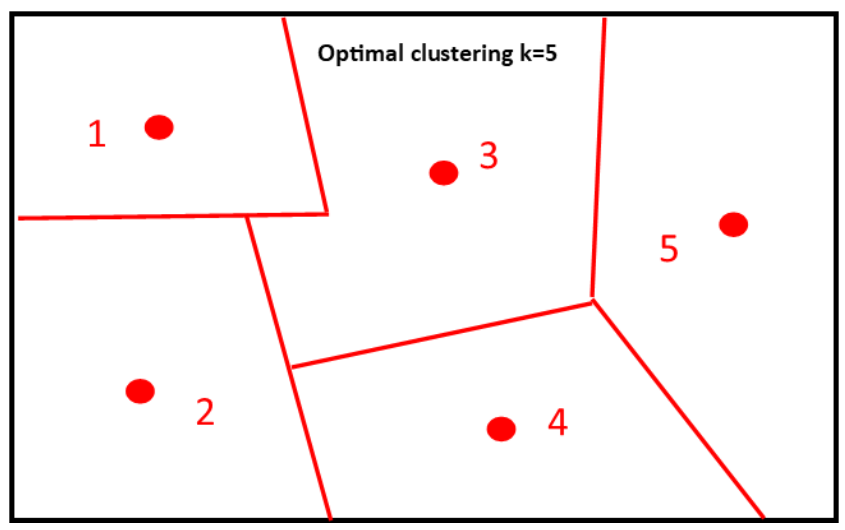
\includegraphics[width=0.8\textwidth]{chapter_1/files/optimal_clustering.png}
    \caption{\small Optimal Clustering with $k=5$}
  \end{figure}			
  \begin{enumerate}
    \begingroup\leftskip4em
  \item[agenda 1.] if the first pick falls under region 2, what
    expected cost for region 2 would be? 
  \item[agenda 2.] if some points are already picked, what expected
    cost for a particular region would be for next pick? 
    \par\endgroup
  \end{enumerate}			
\end{proof}

\begin{lemma}[Lemma 3.2 in $k$-means++ paper]
  Let $A$ be a cluster from $C_{opt}$, let $C$ be just one cluster
  chosen uniformly at random from $A$. Then $\mathbb{E}[\phi(A)]\leq
  2\phi_{opt}(A)$. 
\end{lemma}
\begin{proof}
  \hfill
  \begin{align*}
    \mathbb{E}[\phi(A)] &=\frac{1}{|A|}\sum_{a_0\in A}\sum_{a\in
      A}||a-a_0||^2, \ a_0\text{ is a center that chosen uniformly at
      random from}\ A\\ 
    &= \frac{1}{|A|}\sum_{a_0\in A, a\in
      A}||a-a_0||^2,\  (\textit{recall that
    }\mathbb{E}[||x-y||^2]=2\mathbb{E}[||x-\mathbb{E}(x)||^2])\\ 
    &=2\sum_{a \in A} ||a-\frac{1}{|A|}\sum_{a \in A}a||^2\\
    &=2\sum_{a \in A} ||a-c(A)||^2\\
    &\leq2\phi_{opt}(A)
  \end{align*}
\end{proof}

\begin{lemma}[Lemma 3.3 in $k$-means++ paper]
  Let $A$ be an arbitrary cluster from $C_{opt}$ and $C$ be some
  arbitrary clustering. If we add a random center to $C$ ($C$ is a set
  of centers) from $A$ according to $k$-means++ weighting, then
  $\mathbb{E}[\phi(A)]\leq 8\phi_{opt}(A)$. 
\end{lemma}

\begin{proof}
  \underline{Observation}: probability that $a_0\in A$ is chosen:
  $D^2(a_0)/\sum_{a\in A}D^2(a)$, where $D^2(a_0)= d^2(a_0,C)$ and
  $D(a_0)$ denotes the shortest distance from $a_0$ to the closest
  center we have already chosen.
  
  For a given point $a\in A$, after choosing the center $a_0$, the
  contribution of $a$ to the cost will be $min(D^2(a),
  ||a-a_0||^2)$.\\ 
  \begin{align*}
    \mathbb{E}[\phi(A)] &= \sum_{a_0\in A}\frac{D^2(a_0)}{\sum_{a\in
        A}D^2(a)}\sum_{a\in A} min(D^2(a), ||a-a_0||^2)    \\
    D(a_0)&\leq D(a)+||a-a_0||, \forall a,a_0\\
    D^2(a_0)&\leq (D(a)+||a-a_0||)^2\\
    &\leq 2D^2(a)+2||a-a_0||^2\\
    \sum_{a\in A}D^2(a_0)&\leq 2\sum_{a\in A}(D^2(a)+||a-a_0||^2)\\ 
    D^2(a_0)&\leq \frac{2}{|A|}\sum_{a\in
      A}D^2(a)+\frac{2}{|A|}\sum_{a\in A}||a-a_0||^2\\\\ 
    \mathbb{E}[\phi(A)] &\leq \frac{2}{|A|}\sum_{a_0\in
      A}\frac{\sum_{a}D^2(a)}{\sum_{a}D^2(a)}\sum_{a\in A} min(D^2(a),
    ||a-a_0||^2)\ + \\ 
    &\hspace{1.5em} \frac{2}{|A|}\sum_{a_0\in
      A}\frac{\sum_{a}||a-a_0||^2}{\sum_{a}D^2(a)}\sum_{a\in A}
    min(D^2(a), ||a-a_0||^2)\\ 
    &\text{\textit{(pick}}\ ||a-a_0||^2\ \text{\textit{for the first
        term and pick}}\ D^2(a)\ \text{\textit{for the second
        term.)}}\\ 
    &\leq \frac{4}{|A|}\sum_{a_0\in A}\sum_{a}||a-a_0||^2\\
    &\leq 4\cdot 2\phi_{opt}(A)=8\phi_{opt}(A)
  \end{align*}	
\end{proof}

\begin{lemma}[Lemma 3.4 in $k$-means++ paper]
  Let $C$ be any arbitrary clustering we have chosen, choose $u>0$
  (number of uncovered clustering from $C_{opt}$). The corresponding
  uncovered points are $\chi_u$. Let $\chi_c=\chi-\chi_u$.\\\\ 
  \begin{figure}[H]
    \centering
    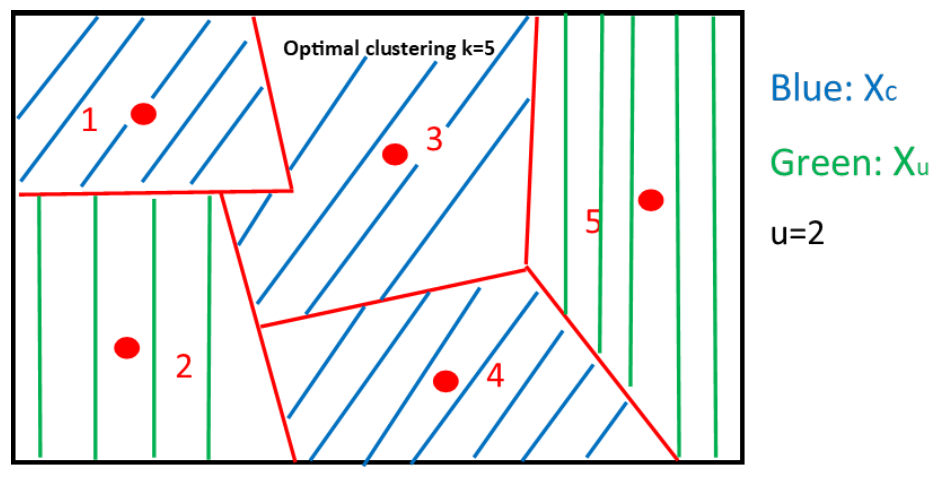
\includegraphics[width=0.8\textwidth]{chapter_1/files/pick_from_uncovered_points.png}
    \caption{\small Optimal Clustering with $k=5$}
  \end{figure}
  Now suppose we add $t\leq u$ random centers (according to
  $k$-means++) and $C'=C\cup\{c_1,c_2\cdots, c_t\}$. The corresponding
  cost is $\phi'$.\\ 
  $$\E[\phi']\leq(\phi(\chi_c)+8\phi_{opt}(\chi_u))(1+H_t)+\frac{u-t}{u}\phi(\chi_u)$$ 
  $$H_t=1+\frac{1}{2}+\frac{1}{3}+\cdots+\frac{1}{t}\ \text{is the harmonic sum}$$
\end{lemma} 

Let $A$ be the cluster which is covered by the first pick. Then
$u=k-1$, chose $t=k-1$ 
\begin{align*}
  \E[\phi']&\leq(\phi(A)+8\phi_{opt}(\chi-A)(1+H_{k-1}),\ (where\ H_{k-1}=2+\log
  k)\\ 
  &= (\phi(A)+8\phi_{opt}-8\phi_{opt}(A))(2+\log k),
  (where\ \phi(A)\leq2\phi_{opt}(A))\\  
  &\leq(2+\log k)8\phi_{opt}		
\end{align*}

\begin{proof}
  The proof was done by induction, showing that if we can prove
  equations $P(u,t-1)$ and $P(u-1,t-1)$ hold true, then $P(u,t)$ holds
  true. Base case of the induction is $P(u,0)\ for\ u>0$ and
  $P(1,1)$. 
\end{proof}

Example: Let $k=3$ for optimal clustering, after first pick there are
2 uncovered clusters from $C_{opt}$. Now we want to prove that
$P(2,2)$ holds true when we pick other two centers with $D^2$
weighting. By induction, if we prove that $P(2,1)$ and $P(1,1)$ hold
true then the result holds.  

Practically it works very well. The initialization is so important that this is always an option when you implement it in your favorite language when you are programming. For example, in Python, k-means++ is the default option. 
	
\subsection{Hartigan's method}

The insight of Hartigan's method is to repeatedly pick a point, and determine its optimal cluster assignment. For $k$ partitions $\{P_j\}_1^k$, the centers $\mu_j = |P_j|^{-1} \sum_{x \in P_j}x$. We also refer to the k-means cost of $P_j$, denoted by $\phi(P_j) = \sum_{x \in P_j} ||x-\mu_j||^2$. For two cluster identity $n, m \in {1,\cdots,k}$, for $x \in P_n$ denote

$$\Delta (i,j,x) = \phi(P_i) + \phi(P_j) - \phi(P_i \backslash \{x\}) - \phi(P_j \cup \{x\}).$$

\begin{algorithm}[H]
  \caption{Hartigan's method}
  \label{ladder-mechanism}
  \begin{algorithmic}[1]
    \renewcommand\algorithmicrequire{\textbf{input}} 
    \REQUIRE ${x_1\cdots x_n}$, $k\in N$
    \STATE Randomly put data $\{x_1\cdots x_n\}$ into $k$ partitions $\{P_1\cdots P_k\}$, and compute ${\mu_j}$
    \STATE Pick any two cluster id $i,j \in \{1,\cdots,k\}$, pick any $x \in P_i$, compute $\Delta(i,j,x)$
    \STATE Choose $j$ to maximize $\Delta(i,j,x)$, and then put $x$ into cluster $P_j$
    \STATE Repeat step 2-3 until no more improvement can be made
  \end{algorithmic}
\end{algorithm}

The algorithm has worse running time, but it always gives us a better final solution.

\subsection{Gaussian Mixture Model (GMM)}
  GMM is a probabilistic modeling technique. As for other techniques, its input is data points $\vec{x}_1, \vec{x}_2, \dots, \vec{x}_n$ from $\bbR^d$ and $k \in \bbN^*$ which 
  is the number of clusters.
  It assumes that there is a probability distribution $\mathcal{D}$ over the joint space $\bbR^d \times [k]$ such that for $(X, C) \sim D$ we have:
  $$\Pr[C = i] = \pi_i$$
  and 
  $$(X | C = i) \sim N(\vec{\mu}_i, \Sigma_i) $$
  Then the assumption is that the data points $(\vec{x}_1, c_1), (\vec{x}_2, c_2), ..., (\vec{x}_n, c_n)$ are drawn iid from a $\mathcal{D}$ but
  that the values of $c_i$ are hidden (or unobserved or unknown).
  
  The task is then to use the observed values $\vec{x}_1, \vec{x}_2, \dots, \vec{x}_n$ to
  estimate the parameters $\pi_1, \vec{\mu}_1, \Sigma_1, \pi_2, \vec{\mu}_2, {\Sigma_2}, ..., \pi_k, \vec{\mu}_k, {\Sigma_k}$.
  
  In other words, the model assumes that the data comes from a mix of $k$ different Gaussian distributions, each with its own mixing component (frequency of points from that
  Gaussian vs from others), its own mean vector (which can be though of as the center of the cluster), and its own covariance matrix (describing the ``tightness'' or ``spread'' of the 
  cluster in all directions).
  
  To estimate the parameters, MLE does not work (when taking the log-likelihood we get the log of a sum which blocks further progress). Instead one can use a heuristic like the 
  Expectation Maximization (EM) algorithm, but this comes with no guarantees. 
  As an interesting side note, there are also more cutting edge techniques that are able to return an arbitrarily good approximation of the true centers 
  of the Gaussians 
  with high probability under some mild assumptions (see ``Learning Mixtures of Gaussians'' by Sanjoy Dasgupta).
  
  As a last note, a nice advantage of this method is that it can give us the probability of a point belonging to a given cluster rather than a 0-1 decision. In some cases this can be very useful.

\subsection{Local Swap Algorithm}	
	The local swap algorithm gives us another very interesting clustering method. The core of the algorithm is to randomly choose $k$ centers,
  and then repeatedly remove a center and replace it with another if that lowers the solution's cost. Here is the exact
  algorithm:
	
\begin{algorithm}[H]
  \caption{Local Swap Algorithm}
  \label{ladder-mechanism}
  \begin{algorithmic}[1]
    \renewcommand\algorithmicrequire{\textbf{input}} 
    \REQUIRE ${x_1\cdots x_n}$, $k\in N$   
    \STATE Pick $T\subset \{x_1\cdots x_n\},\ |T|=k$ 
    \STATE Swap $t_i\in T$ with $x_j\in X$ if it improves the k-means cost.
    \STATE Repeat step 2 until no more improvement can be made.
  \end{algorithmic}
\end{algorithm}

\begin{theorem}[Due to Kanungo et al. '03]
  The cost of the solution returned by the ``local swap method'' is no more than $25+\epsilon$ times the cost of the optimal solution.
  Where $\epsilon$ can be made arbitrarily small.
\end{theorem}
\begin{fact}[Also due to Kanungo et al. '03]
  With some changes the algorithm, the approximation can be brought down to $9+ \epsilon$.
\end{fact}

So the local swap algorithm gives us our first constant factor approximation for the k-means problem!

\subsection{Comparison of heuristics for k-means}
In terms of guarantees, local swap is the best: it gives us a constant factor approximation to the optimal solution. 
Lloyd's algorithm when initialized with the $k$-means++ method has a guarantee that the returned solution won't be worse than $O(\log k)$ times the optimal cost.
This can also be very good for reasonable values of $k$. Hartigan's method and the GMM method do not have guarantees in the general case.

In practice $k$-means++ has an excellent runtime and performance. Hartigan's method seems to give better solutions but takes longer to run. 
GMM is also a very common  choice. The normality assumptions are common in practice, and the runtime and solutions are good. The fact that the model is generative 
and gives probabilities of a point being in each cluster also might be helpful. Local swap is less commonly used in practice, 
mainly due to its high runtime.
	
